\documentclass[twocolumn,10pt]{article}

\usepackage[utf8]{inputenc}
\usepackage[spanish]{babel}
\usepackage[T1]{fontenc}
\usepackage{graphicx}
\usepackage{amsmath,amssymb}
\usepackage{geometry}
\usepackage{hyperref}
\usepackage{booktabs}

\geometry{left=1.6cm, right=1.6cm, top=1.5cm, bottom=1.5cm}
\setlength{\columnsep}{0.5cm}
\setlength{\parskip}{0.4ex}
\setlength{\parindent}{0pt}

\hypersetup{colorlinks=true, urlcolor=blue, linkcolor=black}

\title{\textbf{Control Predictivo Basado en Modelo (MPC)} \\
       \large{para un Sistema Depredador-Presa Aplicado a una App de Citas}}
\author{Emmanuel Guerrero Piza, Kevin Andr\'es Forero Guaitero \\
        \small Cibern\'etica III --- Universidad Distrital, 2026-1}
\date{}

\begin{document}
\twocolumn[
  \maketitle
  \thispagestyle{empty}
]

% ======================================================================
\section{Modelo del sistema}
% ======================================================================

Se modela una aplicaci\'on de citas mediante Lotka-Volterra
($x$: perfiles disponibles, $y$: usuarios activos):
\begin{align}
  \dot{x} &= a\,x - b\,x\,y \label{eq:prey}\\
  \dot{y} &= c\,x\,y - d\,y \label{eq:pred}
\end{align}
Punto de equilibrio: $x^*=d/c$, $y^*=a/b$. Par\'ametros \'optimos
(Parte~2): $a=0.291$, $b=0.0055$, $c=0.0179$, $d=0.700$, con
$x^*\approx39.2$, $y^*\approx53.0$.

\paragraph{Planta estoc\'astica.} Para simular un entorno realista se
incorporan ruido blanco Gaussiano y pulsos aleatorios Poisson:
\begin{align}
  x_{k+1} &= x_k + \Delta t\,(a x_k - b x_k y_k)
            + \sigma_x\varepsilon_x + p_x\delta_{t_P} \notag\\
  y_{k+1} &= y_k + \Delta t\,(c x_k y_k - d y_k)
            + \sigma_y\varepsilon_y + p_y\delta_{t_P} \notag
\end{align}
con $\Delta t=0.1$, $\sigma_x=0.5$, $\sigma_y=0.3$,
$\lambda=0.001$, $p_x\sim\text{Exp}(15)$, $p_y\sim\text{Exp}(5)$,
y $\max(0,\cdot)$ para evitar estados negativos. El MPC desconoce
estos t\'erminos (modelo interno determinista), lo que mide su
robustez ante incertidumbre no modelada.

% ======================================================================
\section{Escenarios de simulaci\'on}
% ======================================================================

Se definen cuatro escenarios sobre la planta estoc\'astica para
evaluar distintas capacidades del controlador (Tabla~\ref{tab:esc}):

\begin{table}[t]
\centering\small
\caption{Definici\'on de los cuatro escenarios de simulaci\'on.}
\label{tab:esc}
\begin{tabular}{@{}llll@{}}
\toprule
\textbf{Esc.} & \textbf{Inicio} & \textbf{Referencia} & \textbf{Particularidad} \\
\midrule
1. Ref.\ cte. & $(40,50)$ & $(35,55)$ fija & Seguimiento b\'asico \\
2. Cambio esc. & $(40,50)$ & $(35,55)\rightarrow(30,58)$ en $t=40$ & Cambio de objetivo \\
3. Perturb. & $(35,55)$ & $(35,55)$ fija & Pulso $+15$ en $x$ en $t=20$ \\
4. Estoc.\ det. & $(40,50)$ & $(35,55)$ fija & Ruido + pulsos (an\'alisis) \\
\bottomrule
\end{tabular}
\end{table}

\textbf{Escenario 1} (referencia constante): el MPC parte de $(40,50)$
y debe alcanzar $(35,55)$. Eval\'ua la capacidad de tracking nominal.
\textbf{Escenario 2} (cambio escal\'on): la referencia cambia
abruptamente de $(35,55)$ a $(30,58)$ en el paso $t=40$ (4~uds.\
de tiempo). Eval\'ua la adaptabilidad del controlador a nuevos
puntos de operaci\'on. \textbf{Escenario 3} (perturbaci\'on): el
sistema parte en equilibrio en $(35,55)$ y recibe un pulso de
$+15$ en $x$ en $t=20$ (2~uds.\ de tiempo), adem\'as del ruido
base. Eval\'ua el rechazo activo a perturbaciones. \textbf{Escenario 4}
(an\'alisis estoc\'astico): 500~pasos con gr\'aficas detalladas de
ruido, pulsos y se\~nal de control para validar la robustez.

Los escenarios 1--3 usan 1000~pasos (100~uds.\ de tiempo) y el
escenario~4 usa 500~pasos.

% ======================================================================
\section{Dise\~no del controlador MPC}
% ======================================================================

\begin{table}[t]
\centering\small
\caption{Par\'ametros de dise\~no del MPC.}
\label{tab:mpc}
\begin{tabular}{@{}ll@{}}
\toprule
\textbf{Par\'ametro} & \textbf{Valor} \\
\midrule
Modelo interno & No lineal (\ref{eq:prey}-\ref{eq:pred}) \\
Horiz. predicci\'on $N$ & 15 pasos \\
Horiz. control $M$ & 10 pasos \\
Pesos $Q$ (estados) & $\text{diag}(1,\;1)$ \\
Pesos $R$ (control) & $\text{diag}(0.1,\;0.1,\;0.1)$ \\
Cotas $a$ (crec.\ perfiles) & $[0.2,\;1.0]$ \\
Cotas $c$ (efic.\ matching) & $[0.002,\;0.04]$ \\
Cotas $d$ (churn) & $[0.1,\;0.7]$ \\
Solver & SLSQP (\texttt{scipy}) \\
Arranque & Warm-start (shift) \\
\bottomrule
\end{tabular}
\end{table}

En cada paso $k$ se resuelve:
\begin{align}
  \min_{\mathbf{u}_{k:M}} &\;
  \sum_{t=0}^{N-1} \bigl[
  \|\mathbf{x}_{k+t+1}\!-\!\mathbf{x}_{\text{ref}}\|_Q^2
  + \|\mathbf{u}_{k+t}\!-\!\mathbf{u}_{\text{ref}}\|_R^2 \bigr] \\
  \text{s.a.}\quad &\mathbf{x}_{k+t+1}=f(\mathbf{x}_{k+t},\mathbf{u}_{k+t}) \\
  &0.2\le a\le1.0,\; 0.002\le c\le0.04,\; 0.1\le d\le0.7
\end{align}
con $\mathbf{x}=[x,y]^T$, $\mathbf{u}=[a,c,d]^T$ y referencia
estacionaria $a_{\text{ref}}=b\,y_{\text{ref}}$,
$d_{\text{ref}}=c_{\text{ref}}\,x_{\text{ref}}$ ($c_{\text{ref}}=0.0179$).

\begin{figure}[t]
  \centering
  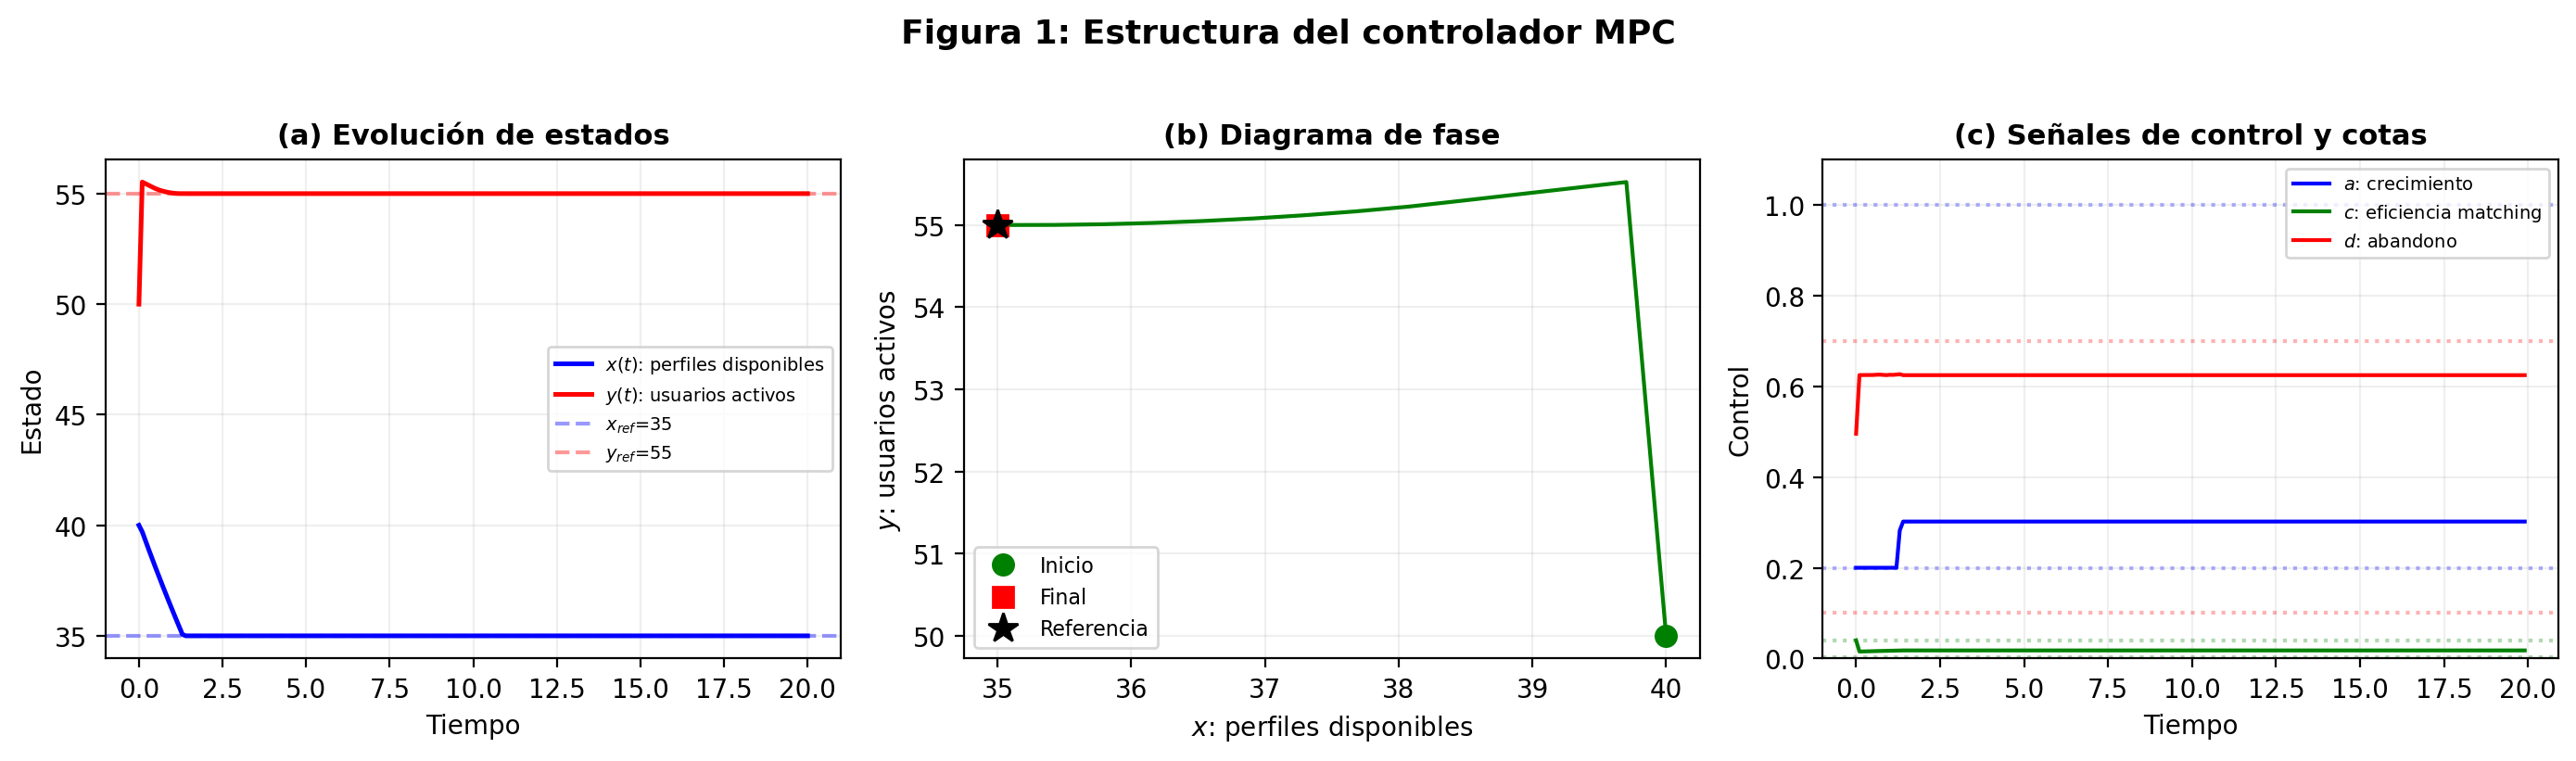
\includegraphics[width=\linewidth]{fig_mpc_estructura.png}
  \caption{Resultado del MPC (Esc.~1, sistema determinista). (a) Los
           estados convergen de $(40,50)$ a $(35,55)$ en $\sim$20~pasos.
           (b) Diagrama de fase: la trayectoria alcanza la referencia.
           (c) Se\~nales de control $a$, $c$, $d$ con cotas (punteadas).}
  \label{fig:mpc}
\end{figure}

La Fig.~\ref{fig:mpc} muestra el comportamiento del MPC con el
sistema determinista. En (a) se observa la convergencia suave de
ambos estados a la referencia en $\sim$20~pasos. En (b), la curva
en el plano de fase conecta el inicio (c\'irculo) con el final
(cuadrado) en la referencia (estrella). En (c), las se\~nales de
control: $a$ se estabiliza en $a_{\text{ref}}=0.30$, $d$ en
$d_{\text{ref}}=0.63$, $c$ en $0.0179$; ninguna viola las cotas
(punteadas). El solver SLSQP alcanza 100\% de \'exito.

% ======================================================================
\section{Resultados sobre la planta estoc\'astica}
% ======================================================================

\begin{figure}[t]
  \centering
  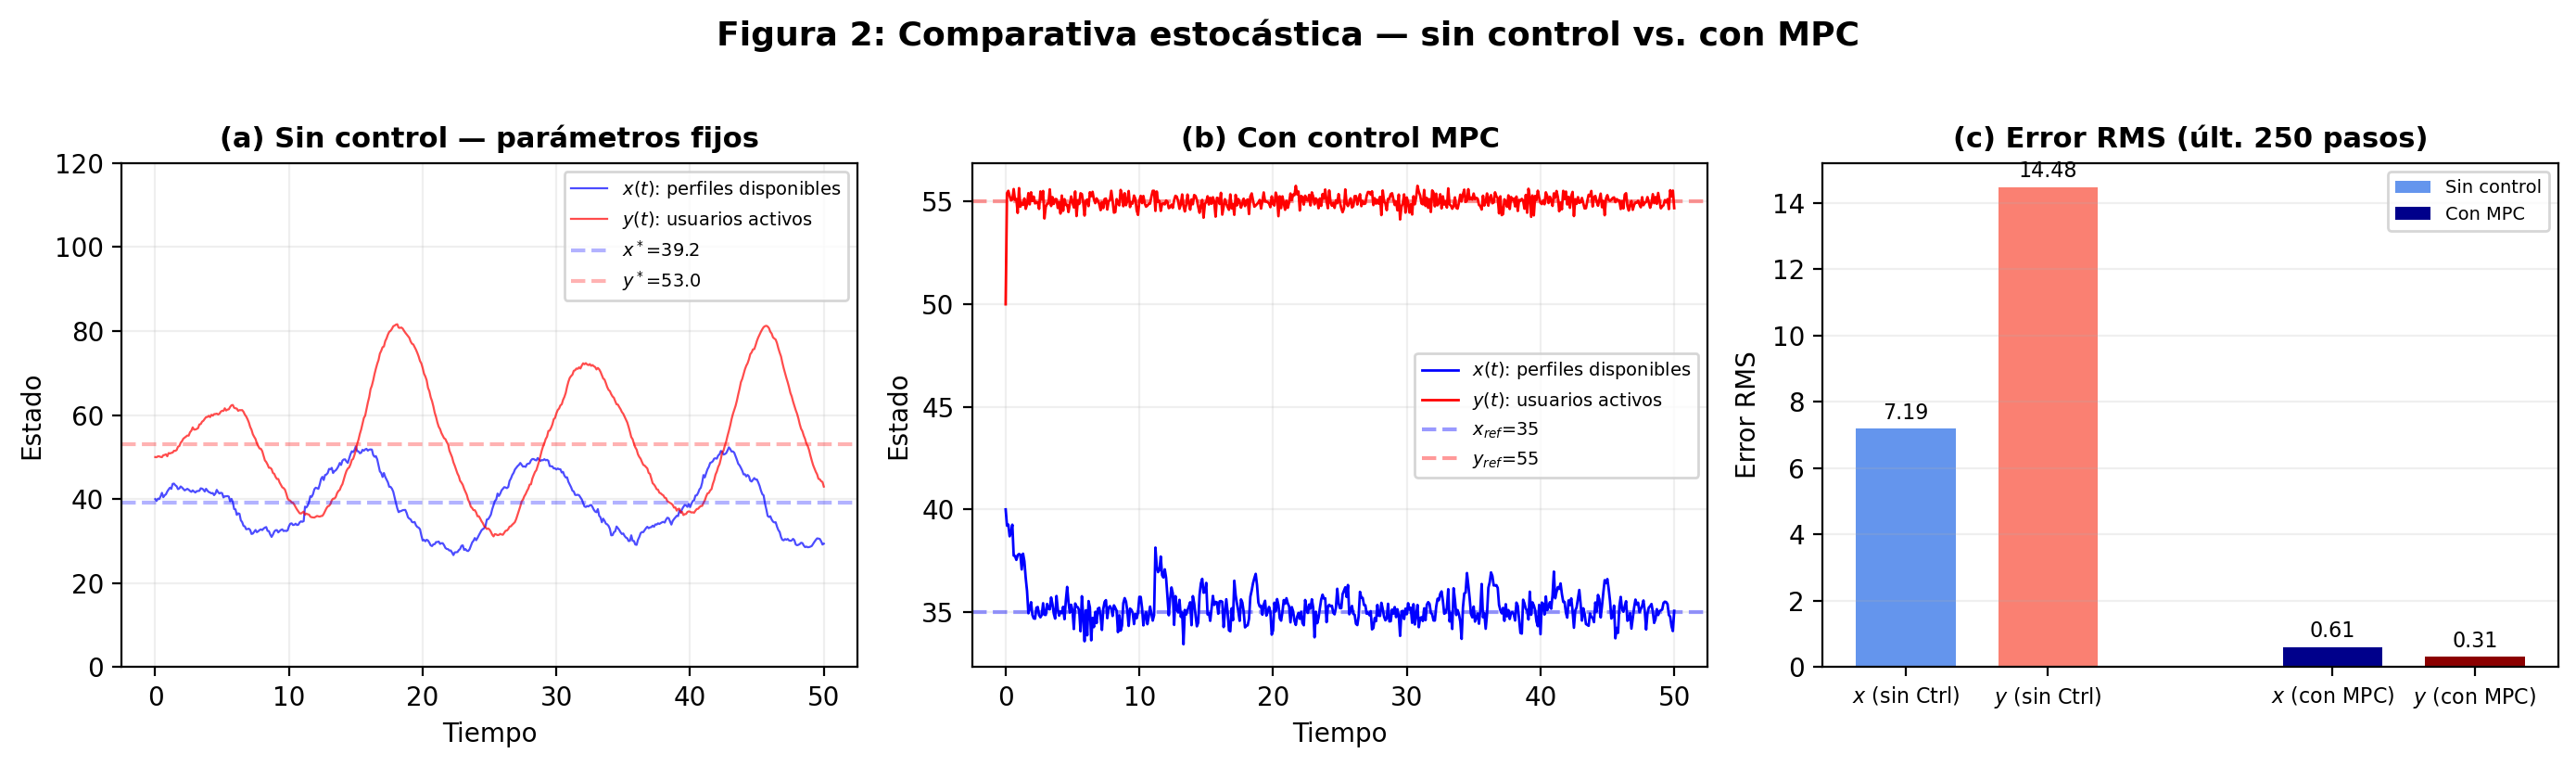
\includegraphics[width=\linewidth]{fig_comparativa_estocastica.png}
  \caption{Comparativa estoc\'astica (Esc.~4, 500~pasos). (a) Sin
           control: estados fluct\'uan alrededor del equilibrio natural.
           (b) Con MPC: el controlador mantiene la referencia. (c)
           Error RMS: mejora $12\times$ ($x$) y $47\times$ ($y$).}
  \label{fig:comp}
\end{figure}

La Fig.~\ref{fig:comp} compara el sistema estoc\'astico sin control
frente al MPC. En (a), los par\'ametros fijos no rechazan el ruido:
los estados oscilan $\pm30$~unidades. En (b), el MPC mantiene ambos
estados cerca de $(35,55)$ pese al ruido y pulsos. En (c), el error
RMS de $x$ pasa de $7.19$ a $0.61$ ($12\times$) y el de $y$ de
$14.48$ a $0.31$ ($47\times$).

La Tabla~\ref{tab:rms} extiende el an\'alisis a los cuatro escenarios.
El error RMS se calcula como $\sigma = \sqrt{\tfrac{1}{N}\sum (x_k -
x_{\text{ref}})^2}$ sobre una ventana estacionaria al final de cada
simulaci\'on, donde el transitorio inicial ya decay\'o.

\begin{table}[t]
\centering\small
\caption{Error RMS (ventana estacionaria).}
\label{tab:rms}
\begin{tabular}{@{}lccc@{}}
\toprule
\textbf{Escenario} & \textbf{Sin control} & \textbf{Con MPC} & \textbf{Mejora} \\
\midrule
1. Ref.\ constante & $\sigma_x=27.13$, $\sigma_y=60.28$ &
  $\sigma_x=1.82$, $\sigma_y=1.57$ & $15\times$, $38\times$ \\
2. Cambio escal\'on & $\sigma_x=6.43$, $\sigma_y=12.92$ &
  $\sigma_x=1.20$, $\sigma_y=0.34$ & $5\times$, $38\times$ \\
3. Perturbaci\'on & $\sigma_x=14.58$, $\sigma_y=31.07$ &
  $\sigma_x=2.82$, $\sigma_y=0.71$ & $5\times$, $43\times$ \\
4. Estoc\'astico & $\sigma_x=7.20$, $\sigma_y=14.45$ &
  $\sigma_x=0.61$, $\sigma_y=0.31$ & $12\times$, $47\times$ \\
\bottomrule
\end{tabular}
\end{table}

En todos los escenarios las restricciones $a\in[0.2,1.0]$,
$c\in[0.002,0.04]$, $d\in[0.1,0.7]$ se respetaron durante toda
la simulaci\'on (ver cotas en Fig.~\ref{fig:mpc}c).

% ======================================================================
\section{Conclusiones}
% ======================================================================

\small
\setlength{\tabcolsep}{3pt}
\begin{tabular}{@{}p{2.8cm}p{2.8cm}p{2.2cm}@{}}
\toprule
\textbf{Requisito gu\'ia} & \textbf{Evidencia} & \textbf{Resultado} \\
\midrule
Ecuaciones modelo & Sec.~1 & LV + estoc\'astico \\
Objetivo control & Sec.~2, Tabla~1 & 4 escenarios \\
Matrices $Q$, $R$ & Tabla~2 & diag(1,1), diag(0.1) \\
Horizontes $N$, $M$ & Tabla~2 & $N=15$, $M=10$ \\
Solver & Tabla~2 & SLSQP, 100\% \'exito \\
Restricciones & Fig.~\ref{fig:mpc}c & 3 cotas respetadas \\
Evol.\ estados & Fig.~\ref{fig:mpc}a & Convergencia ref. \\
Se\~nal control & Fig.~\ref{fig:mpc}c & Cotas respetadas \\
Valid.\ no lineal & Sec.~4 & 4 escenarios \\
Robustez ruido & Fig.~\ref{fig:comp}, Tabla~3 & $5\times$--$47\times$ \\
\bottomrule
\end{tabular}
\normalsize

El MPC no lineal implementado cumple todos los requisitos:
seguimiento de referencia (Fig.~\ref{fig:mpc}), rechazo a
perturbaciones y robustez estoc\'astica (Fig.~\ref{fig:comp}),
con respeto de restricciones.

\end{document}
